% Week 1 Session A — AI-assisted rainfall data reader
% All lab reports in this series include an abstract (see Session A/B .tex).
%
% Build (not printed in the PDF): from this folder run
%   pdflatex Week1_SessionA_Report.tex
% Same folder must contain: week1_session_a.png, week1_session_a_opencode.png,
%   hello_ai.py, prompt_log.md (copy the two code files from
%   ai_water_lab/week1_session_a/ after edits). fvextra is used for wrapped
%   verbatim in the prompt_log appendix.
%
\documentclass[11pt,a4paper]{article}

\usepackage[margin=2.5cm]{geometry}
\usepackage{graphicx}
\usepackage{booktabs}
% Load before hyperref: allows line breaks in \path / \url (underscores, long names)
\usepackage{xurl}
\usepackage{hyperref}
\usepackage{parskip}
\usepackage{enumitem}
\usepackage{xcolor}
\usepackage{listings}
% fvextra extends fancyvrb with breaklines (fixes long lines in prompt_log.md)
\usepackage{fvextra}
\usepackage[most]{tcolorbox}

% --- Fill in your details ---
\newcommand{\studentname}{Your Name}
\newcommand{\studentid}{Your Student ID}
\newcommand{\coursename}{Smart Water Lab / AI-Assisted Development}
\newcommand{\reportdate}{May 15, 2026}

% Allow breaks at spaces inside \path{...} (e.g. "Software Development" in folder names)
\makeatletter
\g@addto@macro\UrlBreaks{\do\ }
\makeatother

% Appendices read from the SAME folder as this .tex (required for Overleaf / cloud
% compilers that do not have ../ai_water_lab/). Keep copies of hello_ai.py and
% prompt_log.md here in sync with your lab folder when you edit them.
\newcommand{\LabCodeRoot}{.}

\lstset{
  basicstyle=\ttfamily\footnotesize,
  breaklines=true,
  breakatwhitespace=true,
  columns=fullflexible,
  keepspaces=true,
  frame=none,
  xleftmargin=0.5em,
  xrightmargin=0.5em,
}

\title{Lab Report: Week 1 Session A\\Environment Setup \& First AI-Generated Script}
\author{\studentname \quad (\studentid)}
\date{\reportdate}

\begin{document}
\maketitle

\begin{abstract}
This report documents the first hands-on session: configuring an AI-assisted development workflow in OpenCode Desktop, generating a Python script with a structured natural-language prompt, executing it locally, and verifying outputs against the assignment requirements. Evidence includes terminal output (Figure~\ref{fig:output}), an OpenCode agent conversation capture (Figure~\ref{fig:opencode}), and full copies of \path{hello_ai.py} and \path{prompt_log.md} in Appendix~\ref{app:hello}--\ref{app:promptlog}.
\end{abstract}

\section{Introduction}
The laboratory introduced a basic collaboration pattern with a coding agent: formulate a clear task, review generated code, run it in a terminal, and record prompts and verification steps. The exercise focused on rainfall data: synthesize a CSV with columns \texttt{date}, \texttt{rainfall\_mm}, and \texttt{location}; read the file with \texttt{pandas}; compute total and average rainfall; and print a short summary report.

\section{Objectives}
The session objectives (from the course guide) were to:
\begin{itemize}[noitemsep]
  \item Set up the development environment (OpenCode Desktop with OpenCode Zen provider).
  \item Generate an initial Python script using AI assistance.
  \item Navigate the IDE (explorer, editor, agent chat, terminal).
  \item Practice documenting prompts and outcomes in a prompt log.
\end{itemize}

\section{Methods}

\subsection{Software and layout}
Work was organized under \path{.../Downloads/Software Development/ai_water_lab/week1_session_a/} (ellipsis stands for your home or project root). OpenCode Desktop (v1.14.50) was used with a connected \textbf{OpenCode Zen} provider and a general-purpose coding model. Python~3 was invoked as \path{python3}; the script depends on \texttt{pandas} and \texttt{numpy}.

\subsection{Prompt used (verbatim)}
The following prompt was sent to the agent:

\begin{quote}\small
I am a water resources student. Please write a Python script that:
\begin{enumerate}[noitemsep]
  \item Creates a sample CSV file with columns: date, rainfall\_mm, location
  \item Reads the CSV file using pandas
  \item Calculates total and average rainfall
  \item Prints a summary report
\end{enumerate}
Include comments explaining each step.
\end{quote}

\subsection{Agent output and local adjustments}
The agent produced a working script, initially saved as \path{rainfall_analysis.py}. The implementation:
\begin{itemize}[noitemsep]
  \item Writes \path{rainfall_data.csv} with 90 records (30 days $\times$ three stations: \path{Station_A}, \path{Station_B}, \path{Station_C}), using an exponential distribution for synthetic daily depths (seeded for repeatability).
  \item Reads the CSV with \texttt{pd.read\_csv}, aggregates by \texttt{location} with \texttt{groupby().agg()} for sum and mean, and prints a formatted report including date span, per-station totals and average daily rainfall, overall mean, and maximum daily value.
\end{itemize}
To match the submission filename in the lab guide, the same code was saved as \path{hello_ai.py}. A separate \path{prompt_log.md} records the prompt, summary, verification, and changes (full text in Appendix~\ref{app:promptlog}).

Figure~\ref{fig:opencode} shows a screenshot of the OpenCode session (prompt and agent response context).

\section{Results}
Running \texttt{python3}~\path{hello_ai.py} completed without errors. The console reported creation of \path{rainfall_data.csv} with 90 records, previewed the first rows, and printed per-station totals (e.g.\ Station\_A: 128.4~mm total; 4.28~mm/day average), overall mean rainfall (4.68~mm/day), and maximum daily rainfall (21.7~mm). Figure~\ref{fig:output} shows the captured terminal output.

\begin{figure}[htbp]
  \centering
  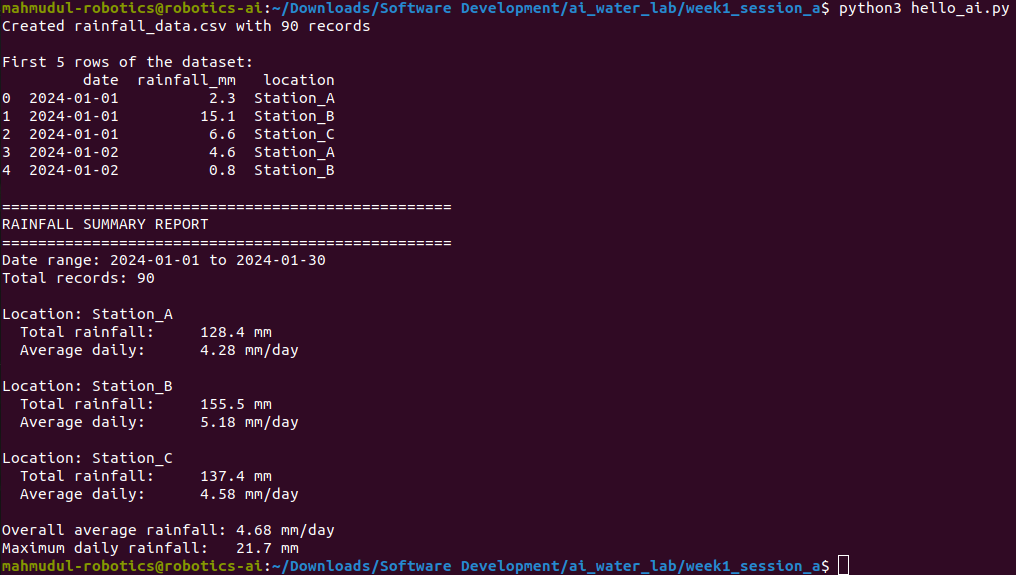
\includegraphics[width=0.95\textwidth]{week1_session_a.png}
  \caption{Terminal output after executing \path{hello_ai.py}: CSV creation, data preview, and rainfall summary report.}
  \label{fig:output}
\end{figure}

\begin{figure}[htbp]
  \centering
  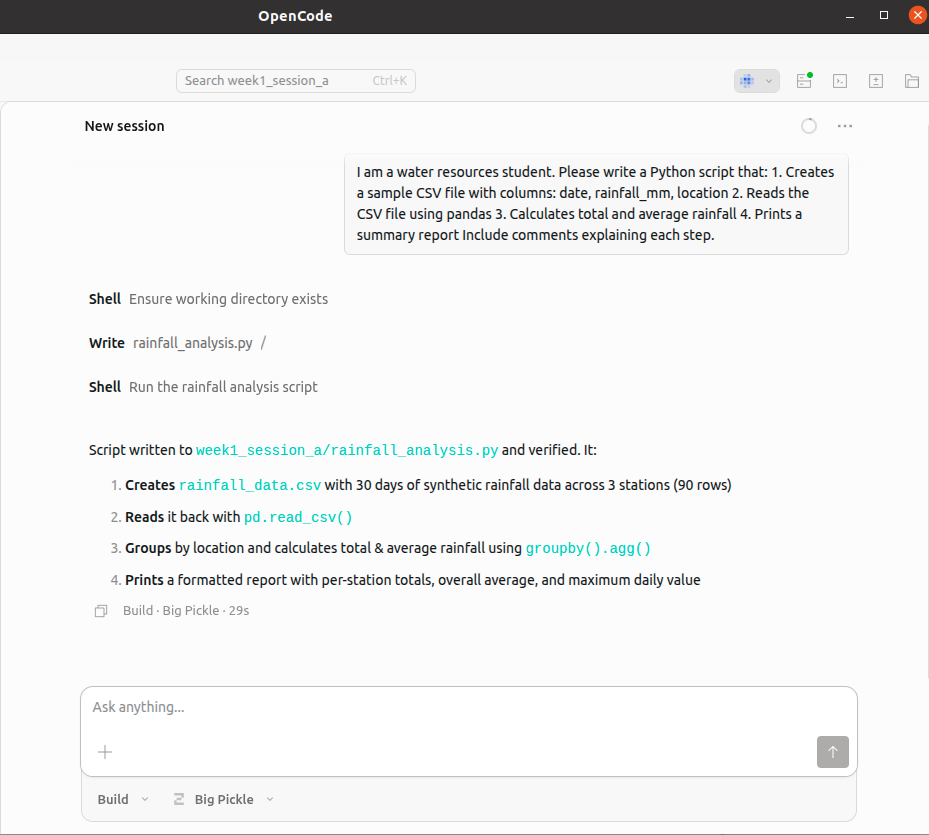
\includegraphics[width=0.95\textwidth]{week1_session_a_opencode.png}
  \caption{OpenCode Desktop: agent conversation showing the lab prompt and generated solution context.}
  \label{fig:opencode}
\end{figure}

\section{Analysis and validation}
\textbf{Structural checks:} The CSV contains the required columns. The script separates creation, read, aggregation, and reporting, with inline comments as requested.

\textbf{Numerical plausibility:} Per-station totals are consistent with summing 30 daily values per station; reported averages equal total divided by 30 for each station. The overall mean is the mean across all 90 rows. Values are non-negative and within a plausible range for synthetic daily depths.

\textbf{Limitations:} Data are synthetic, not observed gauge records, so hydrological conclusions are illustrative only. Random draws could occasionally produce unusually wet or dry spells; the fixed seed improves reproducibility for grading and debugging.

\textbf{Process note:} The agent chose a different default filename than the lab handout: it wrote \path{rainfall_analysis.py} first. The submission uses \path{hello_ai.py}. For future labs, ask explicitly for the output filename in the prompt to avoid renaming.

\section{Problems encountered}
No runtime failures were observed after dependencies were available. The only corrective step was aligning the script filename with the submission checklist by copying to \path{hello_ai.py}.

\section{Lessons learned}
Clear, numbered requirements in the prompt produced runnable code with minimal iteration. Human review still mattered for \emph{deliverable alignment} (file naming) and for confirming that reported statistics match the generated table. Keeping a contemporaneous prompt log makes it straightforward to write this report and to evidence the AI workflow for assessment.

\section{Conclusion}
The session objectives were met: the environment was used end-to-end, a rainfall reader script was generated with AI assistance, executed successfully, and validated at a basic level. This PDF bundles narrative with evidence (Figures~\ref{fig:output}--\ref{fig:opencode}) and full deliverable sources in the appendices. The course portal may still require separate uploads of \path{hello_ai.py}, \path{prompt_log.md}, and image files per the lab guide.

\appendix

\section{Submitted script: \texttt{hello\_ai.py}}
\label{app:hello}
\begin{tcolorbox}[
  enhanced,
  colback=gray!6,
  colframe=black!55,
  title={\texttt{hello\_ai.py} \mdseries (full file)},
  fonttitle=\bfseries\ttfamily\footnotesize,
  arc=1.5mm,
  boxrule=0.7pt,
  breakable,
  width=\linewidth,
  before skip=0.8em,
  after skip=0.8em,
]
\lstinputlisting[language=Python,breaklines=true,breakatwhitespace=false]{\LabCodeRoot/hello_ai.py}
\end{tcolorbox}

\section{Submitted prompt log: \texttt{prompt\_log.md}}
\label{app:promptlog}
\begin{tcolorbox}[
  enhanced,
  colback=gray!6,
  colframe=black!55,
  title={\texttt{prompt\_log.md} \mdseries (full file)},
  fonttitle=\bfseries\ttfamily\footnotesize,
  arc=1.5mm,
  boxrule=0.7pt,
  breakable,
  width=\linewidth,
  before skip=0.8em,
  after skip=0.8em,
]
% breaklines / breakanywhere keep long markdown lines inside the box (needs fvextra)
\VerbatimInput[
  fontsize=\footnotesize,
  breaklines=true,
  breakanywhere=true,
]{\LabCodeRoot/prompt_log.md}
\end{tcolorbox}

\end{document}
